\chapter{A Brief History of Humans \& Stars}
\begin{quote}\em
  That's the wonderful thing about crayons. They can take you to more places than a starship.
\end{quote}
\begin{flushright}
-- Guinan, Star Trek the Next Generation, Season 6, Episode 7.
\end{flushright}
\section{A post prelude prelude}
I will start by saying that I am not trained in history and perhaps it is
self-indulgent to being with such an amateur overview of another academic
field. However, all of the abstraction which we surround ourselves with in so
many of the physical sciences may sometimes sever us from underlying
motivations as to why we are interested. It is true that we often speak to the
public and to funding agencies about grand ambition and infinite possibility;
however, our day-to-day lives are not defined by these things. We spend so much
of our time either immersed in the fine details or proselytizing about greater
purpose that I find that I often feel disconnected from the real reason I am
interested in astronomy. I study astronomy because I am interested in space,
there is no greater reason, nothing more substantial than a five year old
sitting with their father outside their preschool asking about why the stars
and moon are the way that they are. With that being said, please bear with me
as I walk us through a brief history of some of the places stars have had in
human civilization and the evolution of our understanding of them.

\section{Pre-Modern Astronomy}
\subsection{Stars In Ancient Times}
The ancestors of humans have no doubt been looking at the sky since before they
were humans; however, there are limited ways to study these prehistoric
astronomers. Some remnants of early human (pre-history, $\gtrapprox$ 5000 yrs
ago) stargazing to remain, largely in the form of earthen works \addcite. The
earliest records we have show stars playing an important role in religious
practices, navigation, and time keeping \addcite. These early understandings
recognized differences between the fixed stars and the wandering stars though
it would be many more centuries and millennium before the full extent of those
differences became clear \addcite.

As far back as the 1300s B.C.E there were accurate star charts being produced
by ancient Egyptian, Babylonian, and Chinese astronomers. Fourth century B.C.E
Greeks developed star catalogs and many of the modern day English names of stars
still derive from these early catalogs, certain catalogs have either been
rediscovered either in part or in their entirety while others were never 
lost (Figure \ref{fig:starsInHistory}) .

\begin{figure}[htbp]
  \centering
  \begin{subfigure}[t]{0.3\textwidth}
      \centering
      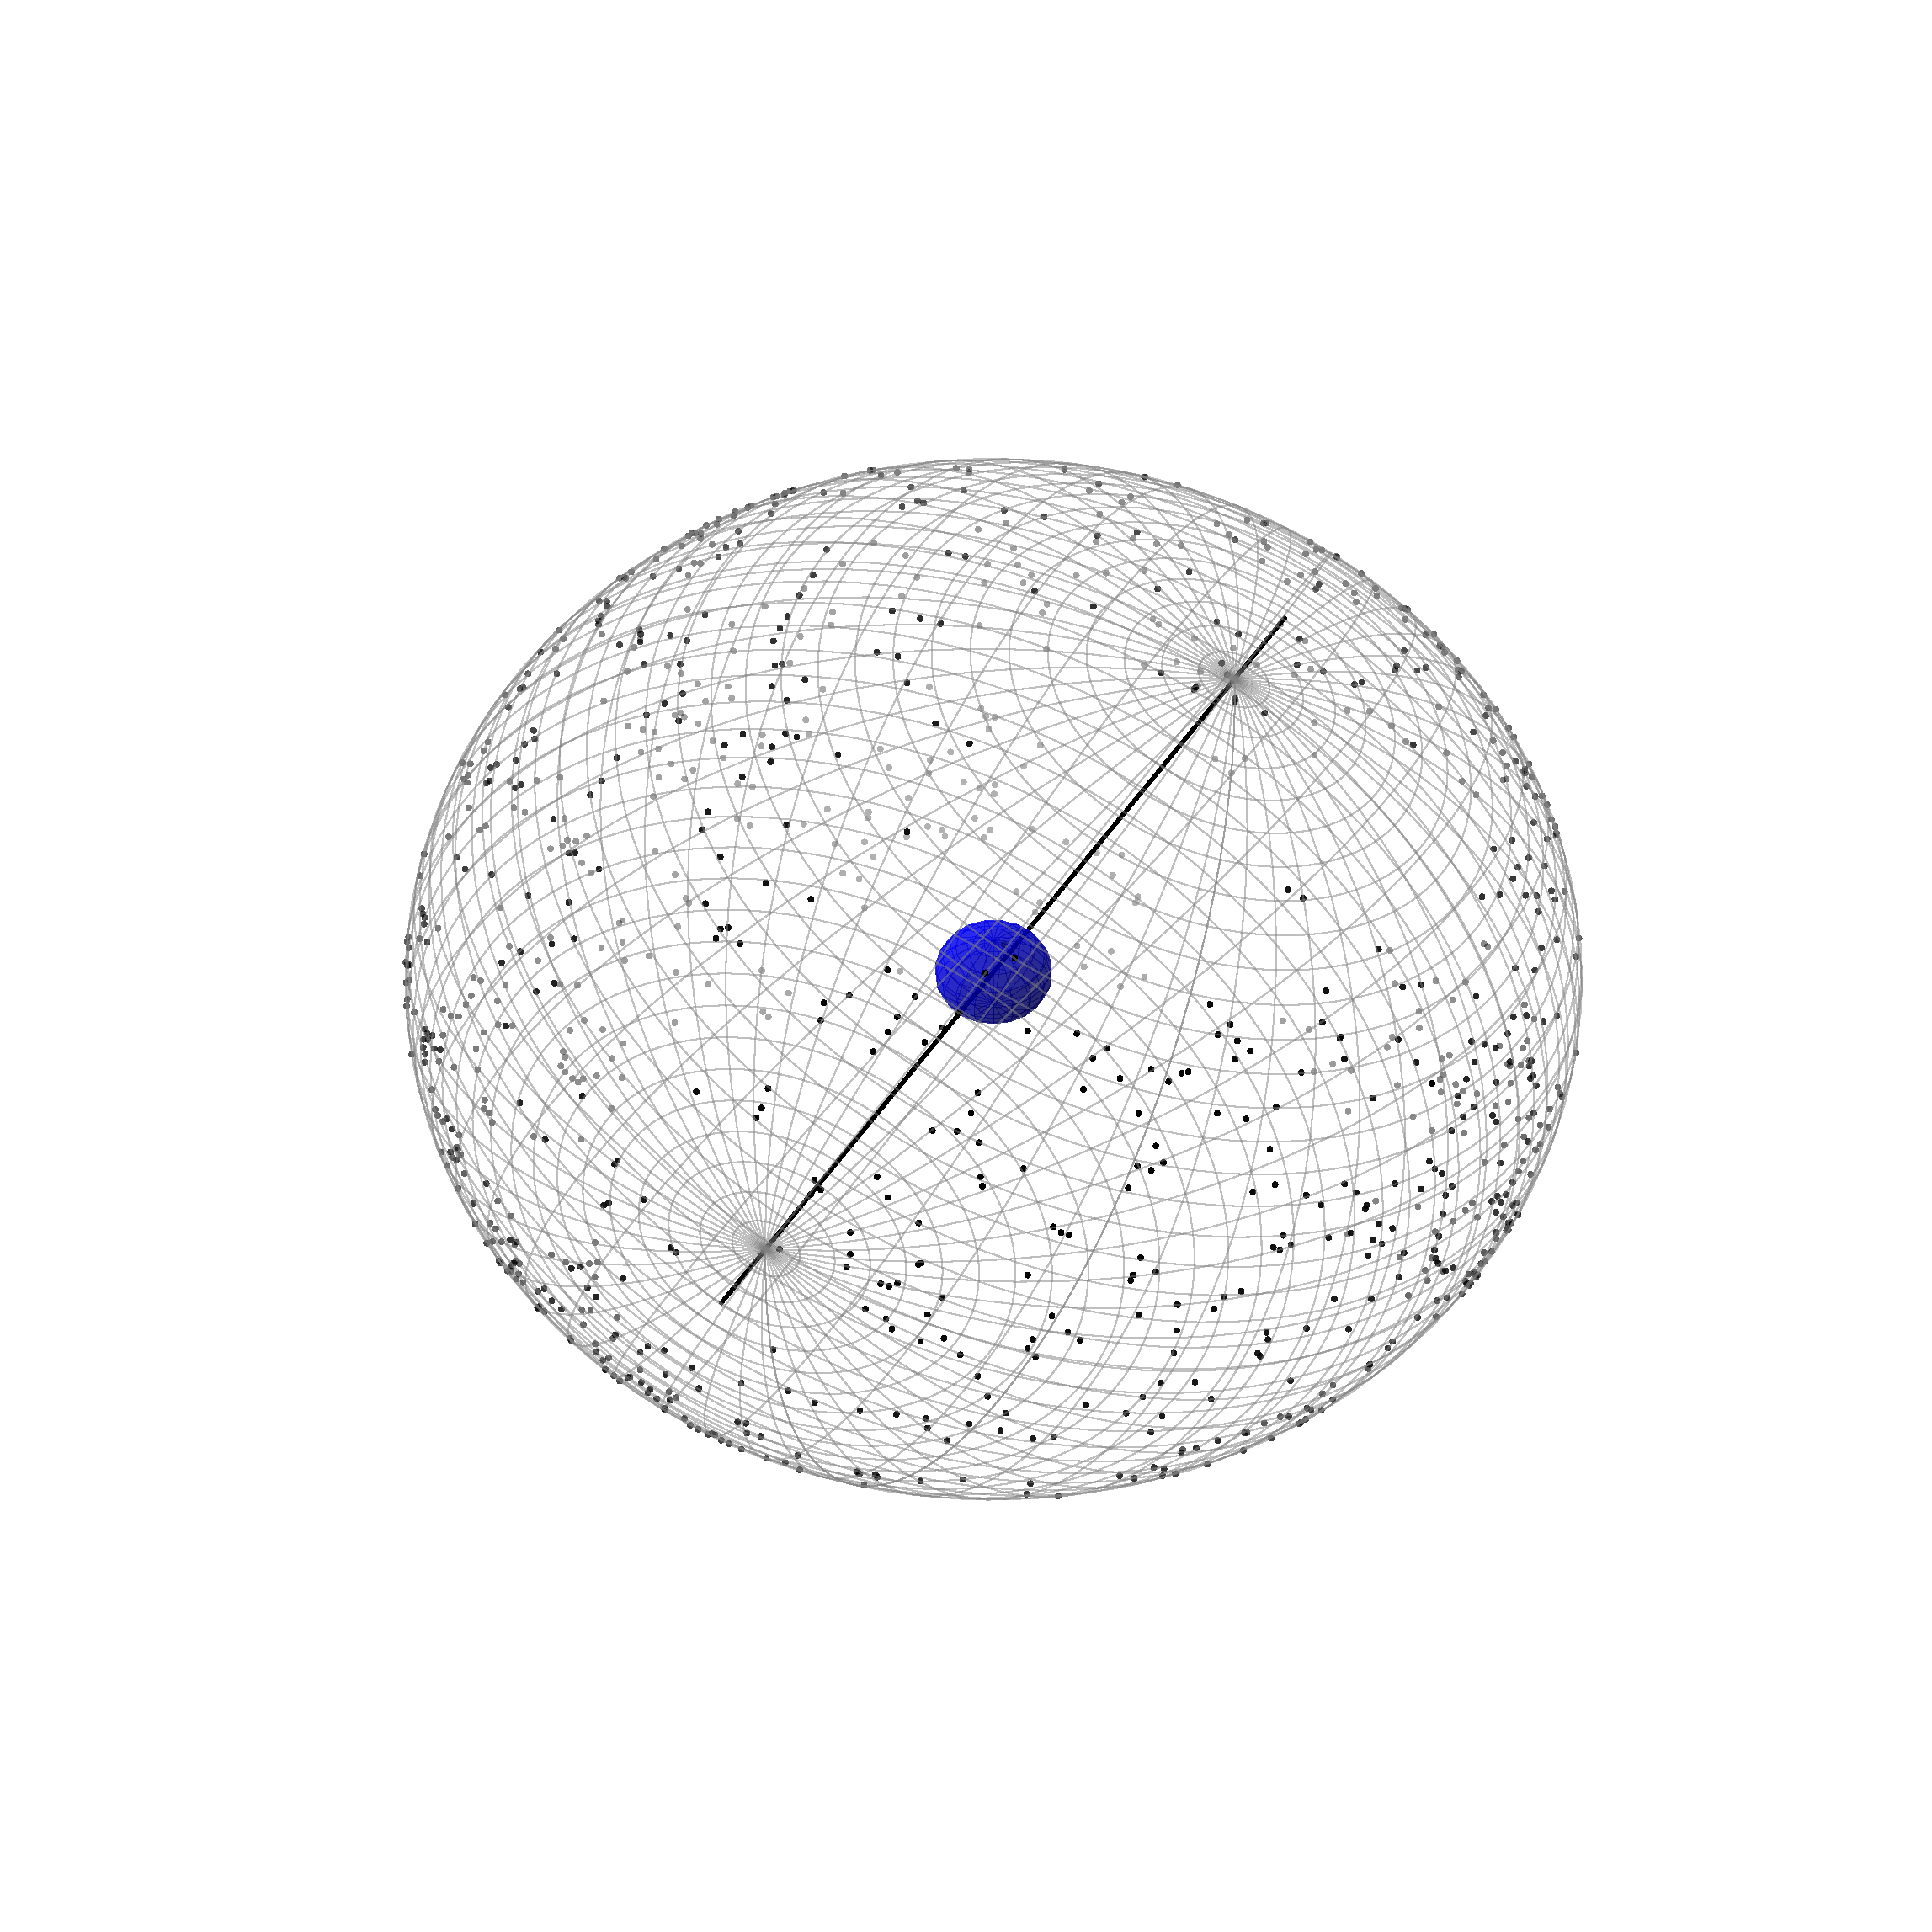
\includegraphics[width=\textwidth]{figures/introduction/Ptolomey.pdf}
      \caption{The stars from Ptolomey's Almegarst projected onto the celestial
      sphere. Coordinates have been updated to the IKRS reference frame.}
      \label{fig:ptolemy}
  \end{subfigure}
  \begin{subfigure}[t]{0.3\textwidth}
      \centering
      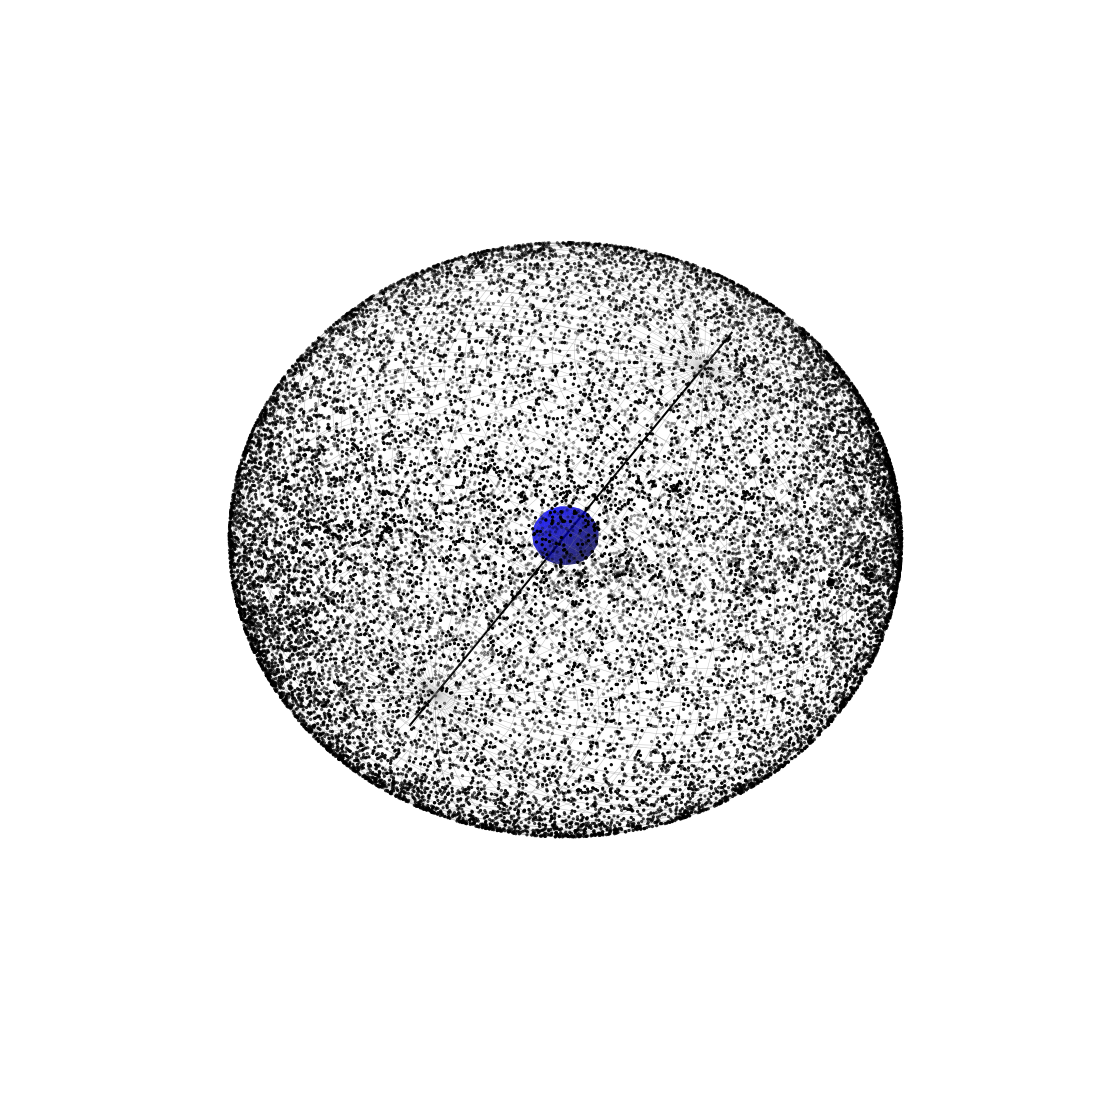
\includegraphics[width=\textwidth]{figures/introduction/ModernStarsGaiaL7.png}
      \caption{Every target in the Gaia DR3 archive with a mean g magnitude
      less than 7. In absolutly perfect conditions these may have been all the
      stars Ptolomey could see.}
      \label{fig:starsL7}
  \end{subfigure}
  \begin{subfigure}[t]{0.3\textwidth}
      \centering
      
\includegraphics[width=\textwidth]{figures/introduction/ModernStarsGaiaL10.png}
      \caption{Every target in the Gaia DR3 archive with a mean g magnitude less than 10. }
      \label{fig:starsL10}
  \end{subfigure}
  \caption{Three variations of the stars on the celestial sphere. Ptolomey did
  not catalogs every visible star; however, his presents one of the earliest
  stellar catalogs which we can still investigate.}
  \label{fig:starsInHistory}
\end{figure}

The understanding of fixed stars at this time was not one of objects similar to
our sun; rather, they were thought to be separate things altogether. Various
cosmologies supposed that stars were points on a celestial sphere which
surrounded the earth, such as the Babylonian cosmology with posited that the
stars existed in a heaven of their own which was interlocked with 2 other
heavens.

\subsection{Astronomy Becomes a Science}
The ancient Greeks, Babylonians, and Chinese contributed to our knowledge of
the positions of heavenly bodies, at least from a earth centric reference
frame; however, it was later work, largely by Islamic and Indian scholars which
form the basis of what we think of as modern astronomy. These astronomers were
not yet conceptualizing the universe the way that we model it today; however,
they began systematized observations of the universe in ways which would be
recognizable. One of the main driving forces of astronomy during this period
was navigation and to that end new instrumentation was developed and early
observatories were built. In 934 C.E. \textit{The Book of Fixed Stars} was
written by Abd al-Rahman al-Sufi. A expansion of the kinds of catalogs which
began over a millennium earlier and allowed for more precise navigation of
ships. 

Potentially more impactful than the creation of new and better catalougs was an
expansion of astronomy from a science of catalouging the positions of bodeis in
the skies to one which could offer insight into the universe. For example, by the 10th
Century C.E. Islamic scholars had found evidence that the Earth was not,
contrary to Ptolomeic ideas, stationary. In the following centuries multiple
criticisms of Ptolemeic theories were published, though none going quite as far
as doubting the geocentric model of the universe. One primary change to these
ancient theories was the recognition that the Earth rotates about its axis as
opposed to the heavens rotating around earth \addcite. 

\subsection{The Birth of Modern Astronomy}
Modern Astronomy does not have a single birth, and different cultures at
different points in time have contributed in various ways to our modern
understanding. Often, in western culture we think of 15th and 16th century
astronomers, such as Johannas Kepler and Tycho Brahe as the first astronomers.
No doubt that Brahe influence pushed the field to systematize certain
observations more and Kepler's theoretical work was some of the earliest which
presented a reasonable model of orbital motion. However, outside of Europe
astronomers such as Uluga Beg \citep[1394 $\rightarrow$ 1449, Figure
\ref{fig:EarlyObvs}][]{sayili1981observatory} and Wang Zehenyi (1768
$\rightarrow$ 1797 \addcite) we building early observatories, improving star catalogs,
and developing models for both lunar and solar eclipses.

\begin{figure}
  \centering
  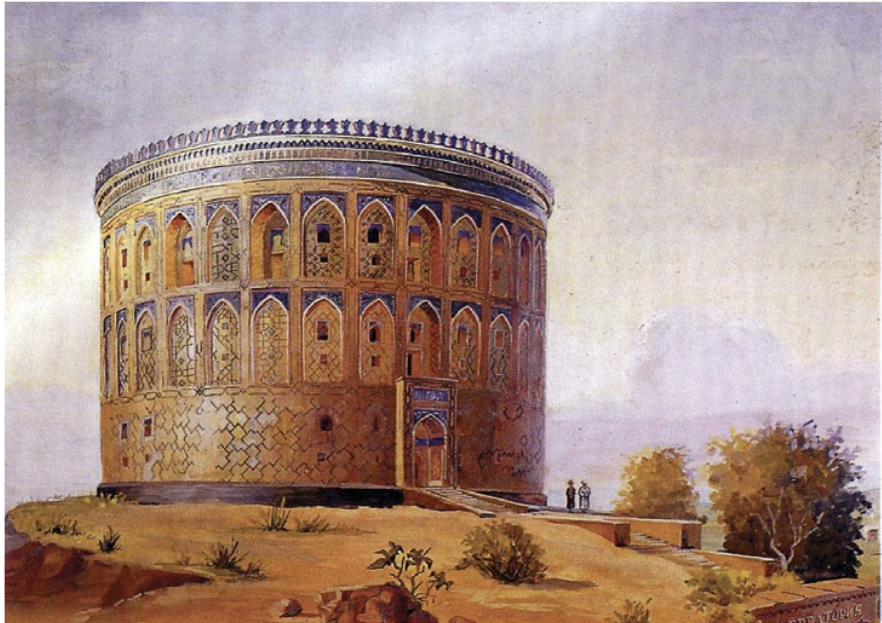
\includegraphics[width=0.85\textwidth]{figures/introduction/EarlyObservatory.png}
  \caption{Artists rendition of the Observatory at Samarkand built by Ulugh Beg
  which was used in the production of the {\em Zij-i Sultani}}
  \label{fig:EarlyObvs}
\end{figure}

Despite Astronomy's extremely long history peoples perceptions of what
stars were had remained relatively fixed over time. There had been some early
astronomers (notably from Aristotle) who proposed that stars might be far away
suns; however, this did not translate to mainstream of global acceptance. This began
to change during the early modern period and it became more common to view stars
as far away stars potentially with their own planetary systems. Even during this
period though, what a star is, what the sun is, physically, was not understood.
